\chapter{Experiments in Simulation}
\label{maintwo}

\section{Simulation Setup} \label{sec:sim_setup}
The experiments of this thesis 
are conducted in a drone racing simulation,
which comprises the drone, the gates that constitute the racetrack
and the scenery.
The implementation of the simulation
is devided into physics modelling and image rendering
(see figure \ref{fig:simulation_setup}).
\begin{figure}[h]
    \centering
    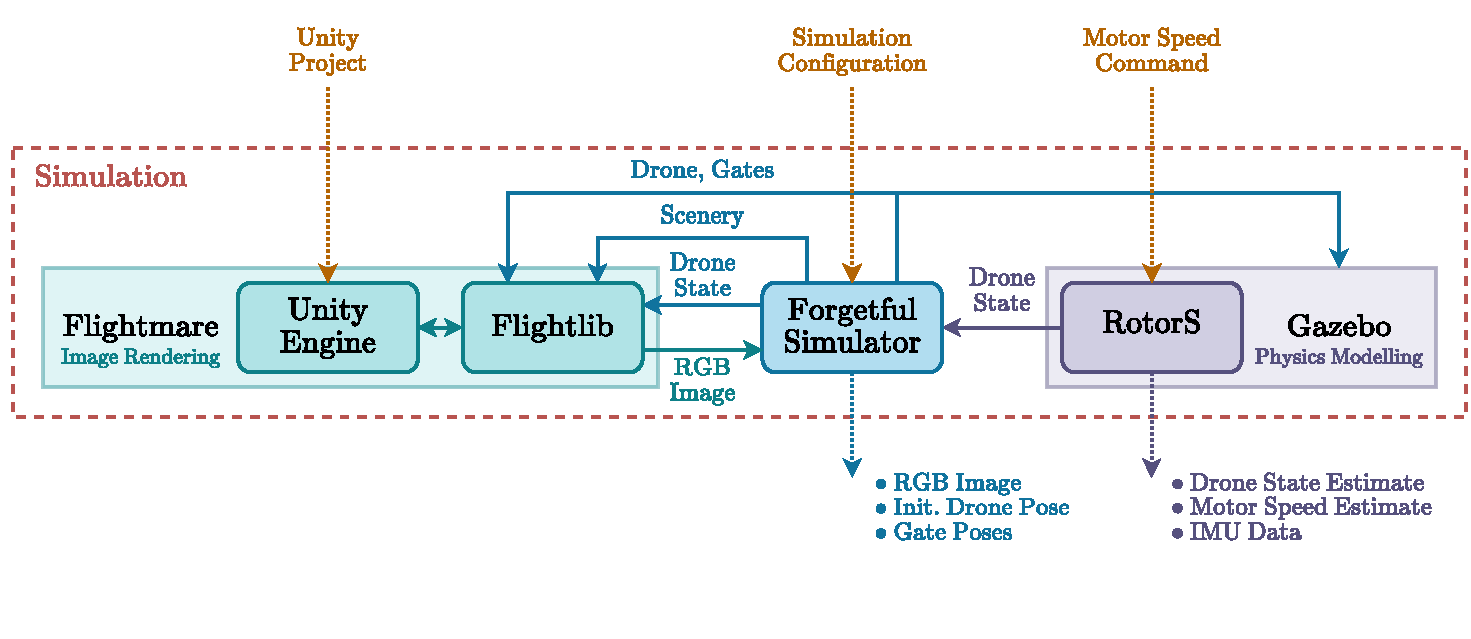
\includegraphics[width=1.0\textwidth]{own/simulation_setup.drawio.pdf}
    \caption[
        Implementation concept of the simulation
    ]{
        Implementation concept of the simulation
    \label{fig:simulation_setup}
    }
\end{figure}

The Gazebo\footnote{
    \url{https://gazebosim.org/home}, visited on 18/08/2022
} 
simulator is deployed to model the physics with high accuracy.
This includes the drone's dynamics and
possible collisions of the drone and the gates.
The RotorS \cite{Furrer2016} plugin
actuates the drone model with the inputted motor speed commands
and outputs the drone state estimate, the motor speed estimate and the data 
from the drone's IMU unit.
%Internally, RotorS sends the ground-truth state to the Forgetful Simulator.
%The 

The Flightmare \cite{Song2020} simulator is deployed to render 
RGB images that are almost photo-realistic.
At a user-specified frequency,
the Flightlib interface
updates the drone's pose, and therewith the drone's onboard camera,
within the Unity\footnote{
    \url{https://unity.com/}, visited on 20/08/2022
} Engine and fetches an RGB image from the onboard camera.
The Unity Engine is built from a Unity project
that bases on the RPG Flightmare Unity Project\footnote{
    \url{https://github.com/uzh-rpg/flightmare_unity}, visited on 20/08/2022
}.
The Unity project
entails five scenes named
spaceship interior\footnote{
    based on "3D Free Modular Kit" from the Unity Asset Store
},
destroyed city\footnote{
    based on "Destroyed City FREE" from the Unity Asset Store
},
industrial site\footnote{
    based on "RPG/FPS Game Assets for PC/Mobile (Industrial Set v2.0)" from the Unity Asset Store
},
polygon city\footnote{
    based on "CITY package" from the Unity Asset Store
}
and desert mountain\footnote{
    based on "Free Island Collection" from the Unity Asset Store
}
(see figure \ref{fig:unity_scenes}).
Each scene has three sites (A, B, C) to place a racetrack.
Two different gate covers, 
one with TU Berlin/DAI-Labor logos and the other with Tsinghua University/DME logos, 
are available (see figure \ref{fig:unity_gates}).
\begin{figure}[h]
    \centering
    \subfloat[
        Spaceship Interior
    ]{
        \label{fig:unity_scene_SI}
        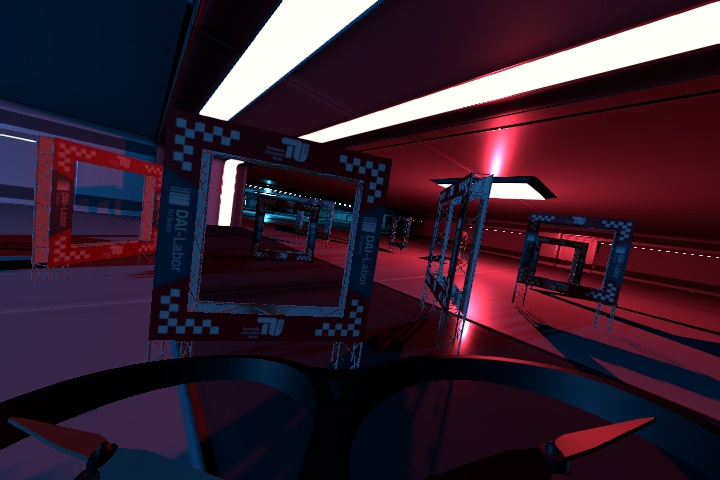
\includegraphics[width=0.33\textwidth]{own/jpg/spaceship_interior.jpg}
    }
    %\hspace*{0cm}                
    \subfloat[
        Destroyed City
    ]{
        \label{fig:unity_scene_DC}
        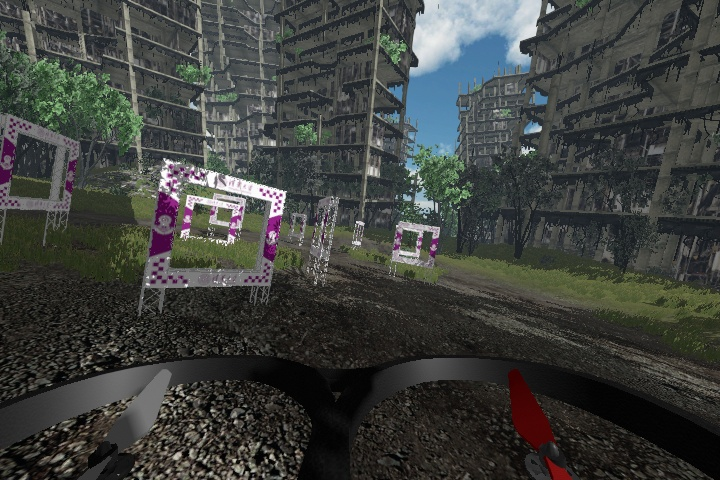
\includegraphics[width=0.33\textwidth]{own/jpg/destroyed_city.jpg}
    }
    \par
    \subfloat[
        Industrial Site
    ]{
        \label{fig:unity_scene_IS}
        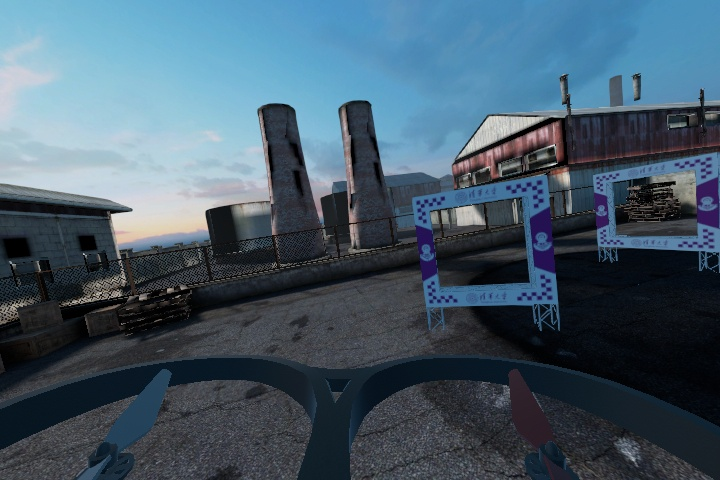
\includegraphics[width=0.33\textwidth]{own/jpg/industrial_site.jpg}
    }
    \subfloat[
        Polygon City
    ]{
        \label{fig:unity_scene_PC}
        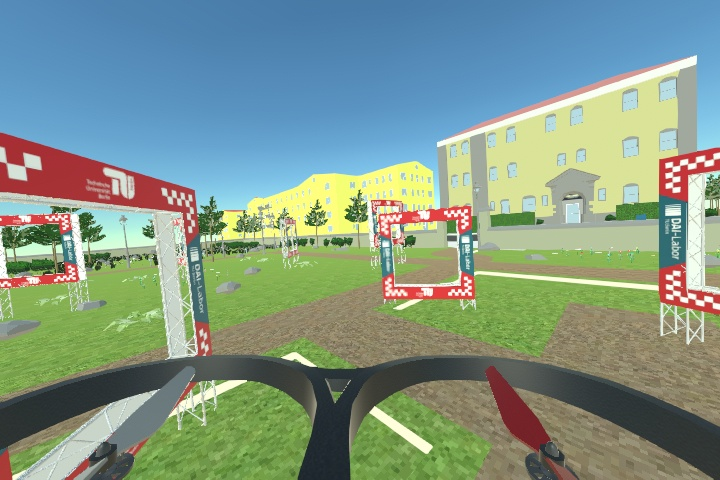
\includegraphics[width=0.33\textwidth]{own/jpg/polygon_city.jpg}
    }
    \subfloat[
        Desert Mountain
    ]{
        \label{fig:unity_scene_DM}
        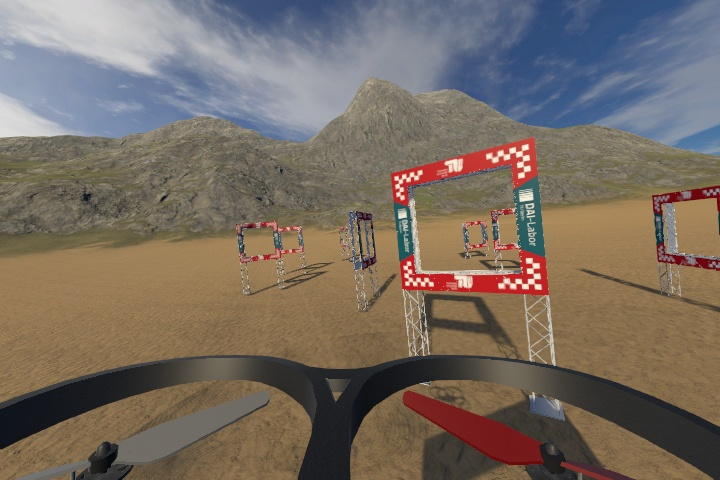
\includegraphics[width=0.33\textwidth]{own/jpg/desert_mountain.jpg}
    }
    \caption[
        Scenes implemented in simulation
    ]{
        Scenes implemented in simulation
        \label{fig:unity_scenes}
    }
\end{figure}
\begin{figure}[h]
    \centering
    \subfloat[
        DAI-Labor at TU Berlin
    ]{
        %\label{fig:unity_scene_SI}
        
\includegraphics[width=0.33\textwidth]{own/jpg/tub_dai_gate.png}
    }       
    \subfloat[
        DME at Tsinghua University
    ]{
        %\label{fig:unity_scene_DC}
        
\includegraphics[width=0.33\textwidth]{own/jpg/thu_dme_gate.png}
    }
    \caption[
        Gate covers implemented in simulation
    ]{
        Gate covers implemented in simulation
        \label{fig:unity_gates}
    }
\end{figure}

The Forgetful Simulator ROS node takes on three tasks.
First, it synchronizes the
drone state in the Flightmare simulator with the
ground-truth state in the Gazebo simulator.
Second, it fetches the RGB images from the Flightmare simulator
and makes them available as output.
Third, it setups the simulation
as requested by the inputted 
simulation configuration as follows.

The simulation configuration specifies the scene
(spaceship interior,
destroyed city,
industrial site,
polygon city or
desert mountain)
, the site (A, B, C),
the gate cover (TUB-DAI or THU-DME) and the racetrack configuration.
The racetrack configuration, in turn, specifies 
the racetrack type (figure-8 or gap), the racetrack generation (deterministic or randomized) 
and the racetrack direction (clockwise or counterclockwise).
The Forgetful Simulator, 
which stores the data of the deterministic, 
counterclockwise gate poses
of the available racetrack types (see table \ref{tab:gate_pos}), 
processes the racetrack configuration as shown in figure
\ref{fig:racetrack_comp}.
If specified,
the generation of the racetrack is randomized.
The randomization starts from 
the stored gate poses of the specified racetrack type
and includes the following steps.
\begin{enumerate}
    \item This step only applies to the gap racetrack type
    as it explicitely randomizes the gap distance.
    Sample the y-position values 
    of the gates \#3-6 from the uniform real distribution
    over the intervals specified in table \ref{tab:gate_pos}.
    
    \item Shift the gate positions along the $x$-, $y$- and $z$-axis
    by a value, which is sampled, 
    independently for each gate and axis, 
    from the uniform real distribution
    over the user-specified interval 
    $\left[
        -\dist[\user]{\text{sim}}{\text{shift},\mxm}{}{},
        \dist[\user]{\text{sim}}{\text{shift},\mxm}{}{}\right]$.
    
        \item Scale all gate positions by the same value
    sampled from the uniform real distribution
    over the user-specified interval
    $\left[
        \dist[\user]{\text{sim}}{\text{shift},\mnm}{}{}, 
        \dist[\user]{\text{sim}}{\text{shift},\mxm}{}{}\right]$.
    \item Twist the gate yaw-orientations
    by a value, which is sampled, 
    independently for each gate, 
    from the uniform real distribution
    over the user-specified interval
    $\left[
        -\dist[\user]{\text{sim}}{\text{twist},\mxm}{}{},
        \dist[\user]{\text{sim}}{\text{twist},\mxm}{}{}\right]$.
\end{enumerate}
Further, if specified, the gate poses
are redirected from counterclockwise to clockwise.
The drone's start position is computed so that
the drone is located 
between the second last and the last gate
and faces towards the last gate.
After processing the racetrack configuration,
the Forgetful Simulator loads the specified scene and site in 
the Flightmare Simulator and spawns the drone model 
and the gate models (with the specified cover)
at the computed poses
in both, the Flightmare and the Gazebo, simulator.
Finally, the Forgetful Simulator
outputs the computed initial drone and gate poses,
which for example are required by the expert system.




\begin{figure}[h]
    \newcommand{\dimmm}{0.42\textwidth}
    \newcommand{\dimmmb}{0.1\textwidth}
    \newcommand{\vertspace}{-3ex}

    \centering
        \subfloat{\footnotesize \textbf{$\downarrow$ shift}}
    \\[\vertspace]
        \subfloat{
            %\fbox{
                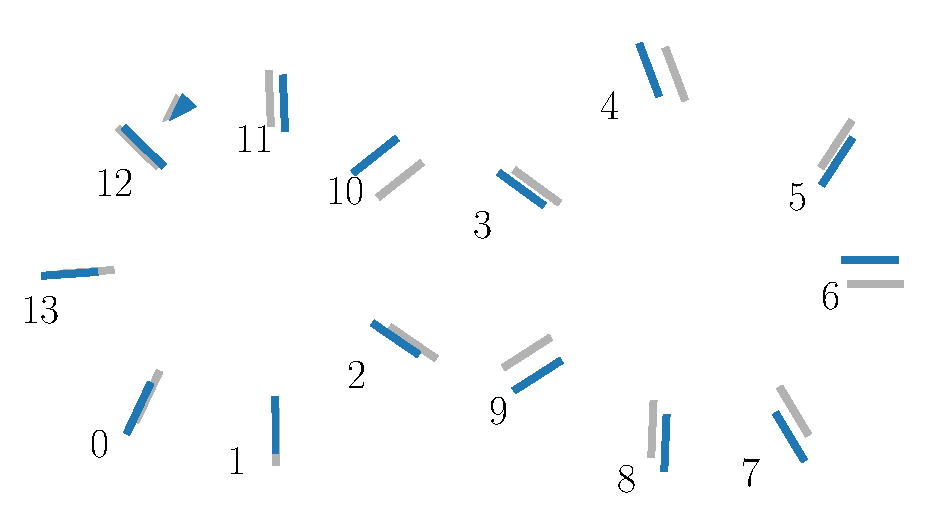
\includegraphics[width=\dimmm]{own/computeRacetrack_fig8_shift.pdf}
            %}
        }
        \subfloat{\begin{minipage}[c]{\dimmmb}$\ $\end{minipage}}
        \subfloat{
            %\fbox{
                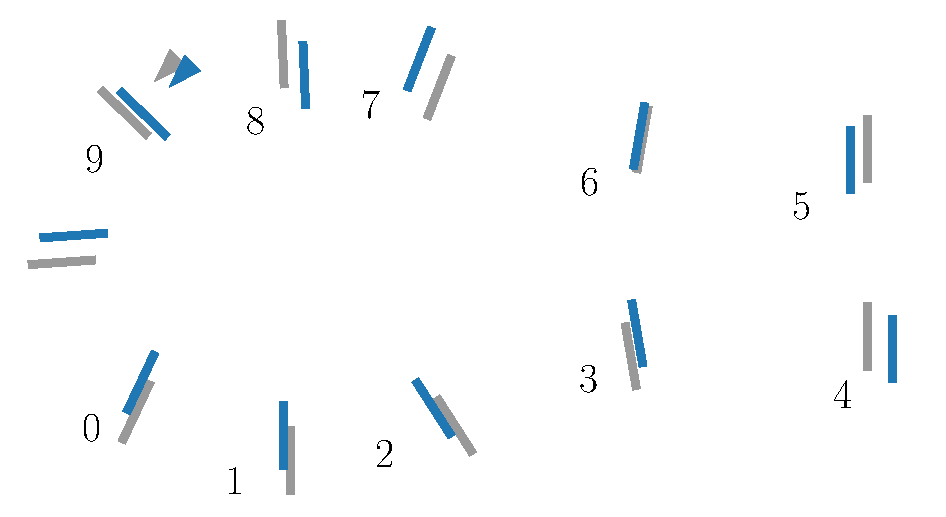
\includegraphics[width=\dimmm]{own/computeRacetrack_gap_shift.pdf}
            %}
        }
    \\[\vertspace]
        \subfloat{\footnotesize \textbf{$\downarrow$ scale}}
    \\[\vertspace]
        \subfloat{
            %\fbox{
                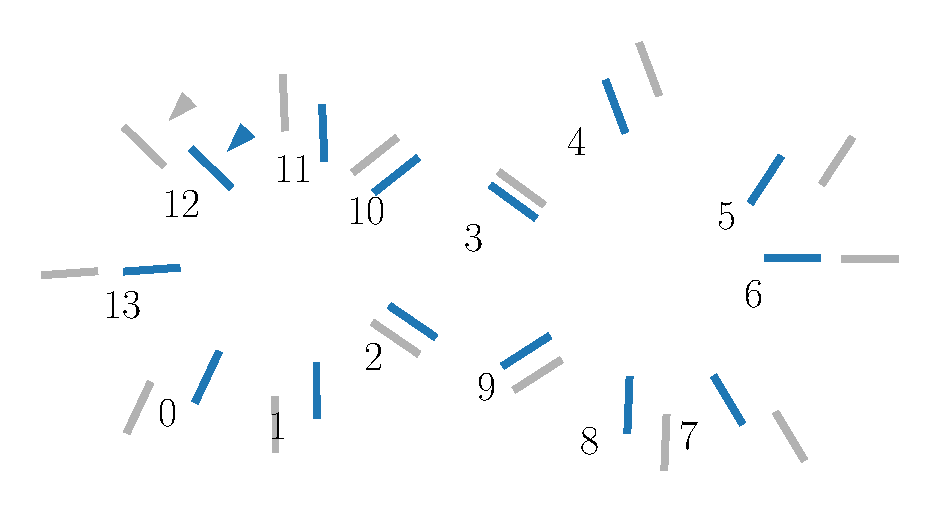
\includegraphics[width=\dimmm]{own/computeRacetrack_fig8_scale.pdf}
            %}
        }
        \subfloat{\begin{minipage}[c]{\dimmmb}$\ $\end{minipage}}
        \subfloat{
            %\fbox{
                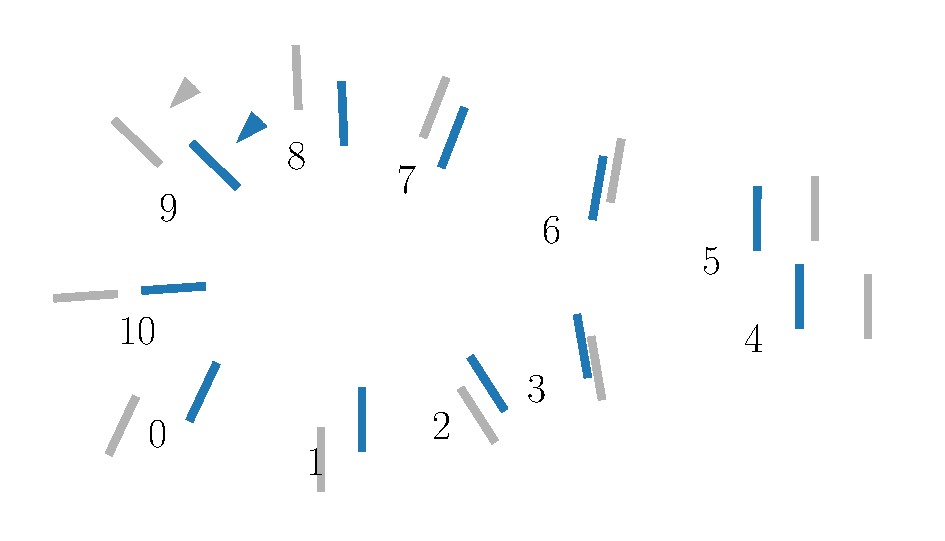
\includegraphics[width=\dimmm]{own/computeRacetrack_gap_scale.pdf}
            %}
        }
    \\[\vertspace]
        \subfloat{\footnotesize \textbf{$\downarrow$ twist}}
    \\[\vertspace]
        \subfloat{
            %\fbox{
                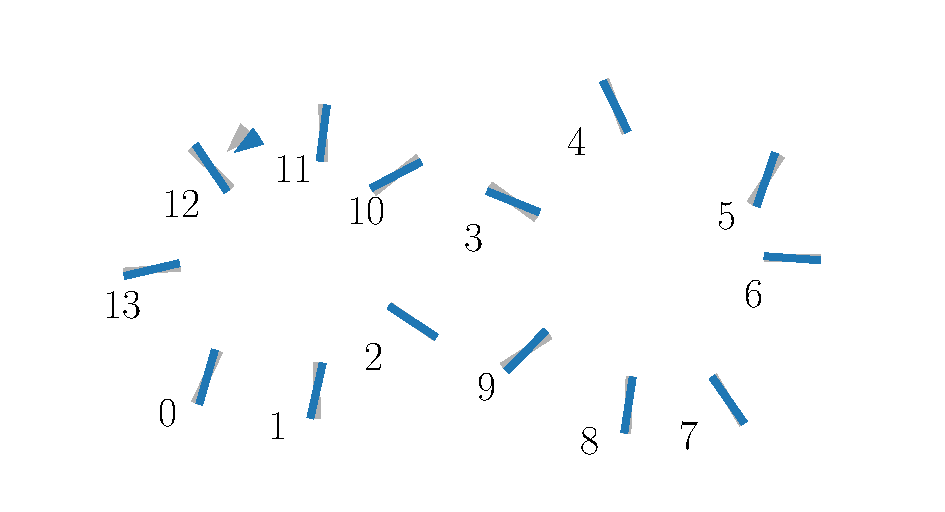
\includegraphics[width=\dimmm]{own/computeRacetrack_fig8_twist.pdf}
            %}
        }
        \subfloat{\begin{minipage}[c]{\dimmmb}$\ $\end{minipage}}
        \subfloat{
           %\fbox{
            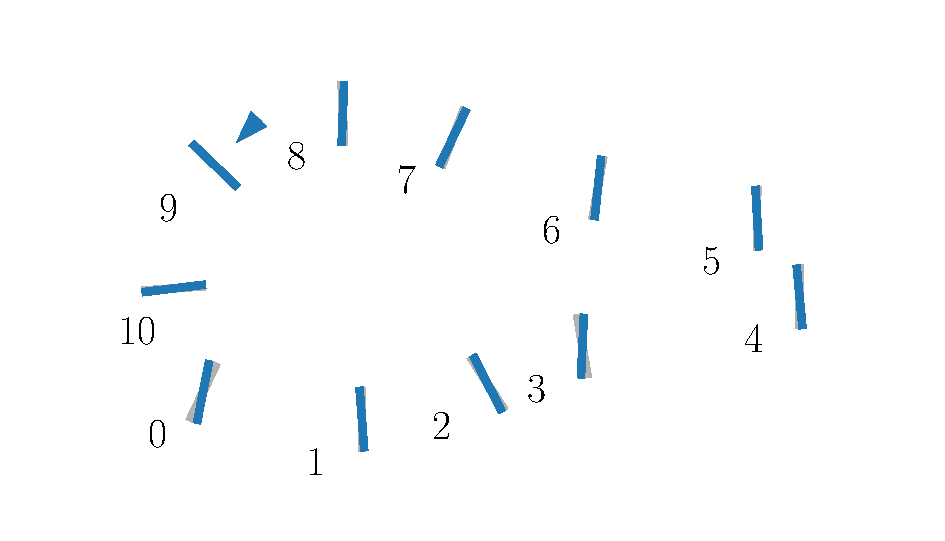
\includegraphics[width=\dimmm]{own/computeRacetrack_gap_twist.pdf}
        %}
        }
    \\[\vertspace]
        \subfloat{\footnotesize \textbf{$\downarrow$ redirect}}
    \\[\vertspace]
    \subfloat{
        %\fbox{
            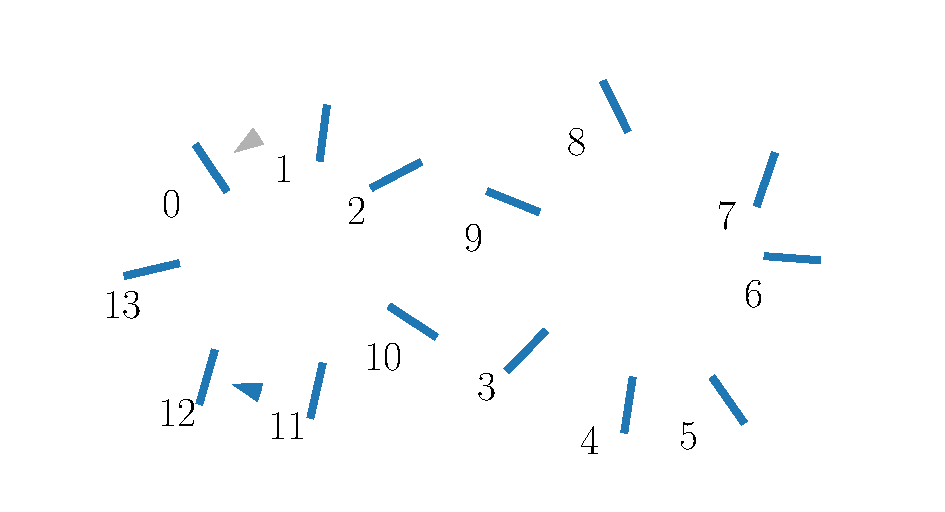
\includegraphics[width=\dimmm]{own/computeRacetrack_fig8_redir.pdf}
        %}
    }
    \subfloat{\begin{minipage}[c]{\dimmmb}$\ $\end{minipage}}
    \subfloat{
        %\fbox{
            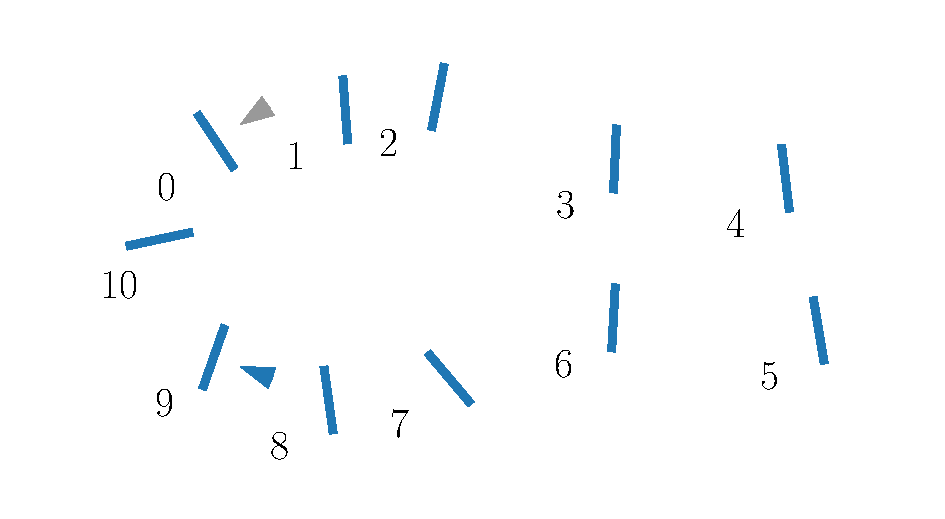
\includegraphics[width=\dimmm]{own/computeRacetrack_gap_redir.pdf}
        %}
    }
    \caption[
        Processing of the racetrack configuration
    ]{
        Processing of the racetrack configuration for
        the figure-8 (left) 
        and the gap (right) racetrack type.
        In the xy-plane, the drone's starting pose (arrow) and the gate poses 
        (numbered bars)
        are depicted before (grey) and after (blue) the individual processing step.
        The randomizing processing step, which is exclusive to the gap racetrack type,
        is not shown.
        \label{fig:racetrack_comp}
    }
\end{figure}







\begin{table}[h]
    \footnotesize
    \caption{Deterministic gate poses\label{tab:gate_pos}}
    \centering
    \begin{tabular}{|l|l|l|l|l|l|}
    %\hline
    %\multicolumn{3}{|c|}{Team sheet} \\
    \hline
    Racetrack & Gate & x & y & z & yaw\\ 
    \hline
    \hline
    \multirow{14}{*}{Figure-8}   
    &0 &-20.45& -8.65&2.0& 1.13\\ \cline{2-6}
    &1 &-12.55&-11.15&2.0&-1.57\\ \cline{2-6}
    &2 &-4.15 & -5.35&2.0&-0.60\\ \cline{2-6}
    &3 &3.45  &  4.25&2.0&-0.63\\ \cline{2-6}
    &4 &11.95 & 11.15&2.0&-1.21\\ \cline{2-6}
    &5 &21.85 &  6.85&2.0& 0.99\\ \cline{2-6}
    &6 &24.25 & -1.75&2.0& 0.00\\ \cline{2-6}
    &7 &19.25 & -9.55&2.0&-1.03\\ \cline{2-6}
    &8 &10.55 &-10.65&2.0& 1.53\\ \cline{2-6}
    &9 &2.85  & -5.95&2.0& 0.57\\ \cline{2-6}
    &10&-4.95 &  4.65&2.0& 0.67\\ \cline{2-6}
    &11&-12.95&  9.65&2.0&-1.53\\ \cline{2-6}
    &12&-21.05&  6.65&2.0&-0.77\\ \cline{2-6}
    &13&-24.25& -1.00&2.0& 0.07\\
    \hline
    \hline
    \multirow{14}{*}{Gap}   
    &0 &-20.45&-8.65         &2.0& 1.13\\ \cline{2-6}
    &1 &-12.55&-11.15        &2.0&-1.57\\ \cline{2-6}
    &2 &-4.15 &-9.35         &2.0& -1.0\\ \cline{2-6}
    &3 &4.85  &[-4.95, -5.95]&2.0& -1.4\\ \cline{2-6}
    &4 &16.95 &[-2.25, -5.25]&2.0& 1.57\\ \cline{2-6}
    &5 &16.95 &[2.25,   5.25]&2.0& 1.57\\ \cline{2-6}
    &6 &5.45  &[4.45,   5.45]&2.0&  1.4\\ \cline{2-6}
    &7 &-4.95 &7.95          &2.0&  1.2\\ \cline{2-6}
    &8 &-12.95&9.65          &2.0&-1.53\\ \cline{2-6}
    &9 &-21.05&6.65          &2.0&-0.77\\ \cline{2-6}
    &10&-24.25&-1.0          &2.0& 0.07\\
    \hline
    \end{tabular}
\end{table}






\section{ANN Module Variants}
In the experiments, several
variants of the ANN module (see section \ref{sec:ann_module})
are examined for their racing performance.
Table \ref{tab:ann_module_variants} shows these variants
and their configurations.
The configuration of a variant
is structured into
input, output and the 
CNN, GRU, FC, and HEAD submodule.

The input configuration includes:
the sequence length $\seqLen$ of the training samples 
(see equ. \ref{eq:seq_len}),
the resize factor $\resizeFact$ 
of the image preprocessing (see equ. \ref{eq:rgb_preproc})
as well as the switchable optional inputs
$\rawRGBTimeStep$, 
$(\IMULinAcc,\IMUAngVel)$
and
$\IMUTimeStep$ (see equ. \ref{eq:opt_inp_vec}).
The output configuration includes:
navigation decision
$\headNavDec$ (see equ. \ref{eq:head_nav_dec})
and control command
$\headCtrlCmd$ (see equ. \ref{eq:head_ctrl_cmd}).
For the
configurations regarding the CNN, GRU, FC and HEAD submodules,
see the corresponding paragraphs in section \ref{sec:ann_module}. 


%All of the examined variants have three configurational aspects in common.
%First, all available optional inputs are activated.
%Second, navigation decisions are selected as output option.
%Third, the CNN submodule implements the backbone of the ResNet18 PyTorch implementation
%whose parameters are trainable and pretrained on ImageNet !!!.
%The ResNet18 contains 18 layers and has ... trainable parameters ...

\newcommand{\numColumns}{5}
\begin{table}[h]
    \caption{ANN module variants\label{tab:ann_module_variants}}
    \centering
    \begin{tabular}{|l|l|l|l|l|} \hline
                        &                           &Baseline    &Baseline+     & Sequential \\\hline\hline
\multirow{5}{*}{Input}  &$\seqLen$                  &1           &1             &$\setOfInts{2,3,5,10,25}$             \\\cline{2-\numColumns}
                        &$\resizeFact$              &\sfrac{1}{2}&\sfrac{1}{2}  &$\setOfInts{\sfrac{1}{2}, \sfrac{1}{3}}$   \\\cline{2-\numColumns}
                        &$\rawRGBTimeStep$          &\xmark      &\cmark        &\cmark         \\\cline{2-\numColumns}
                        &$(\IMULinAcc,\IMUAngVel)$  &\xmark      &\cmark        &\cmark         \\\cline{2-\numColumns}
                        &$\IMUTimeStep$             &\xmark      &\cmark        &\cmark         \\\hline
\multirow{1}{*}{Output} &$\headNavDec$              &\cmark      &\cmark        &\cmark         \\\cline{2-\numColumns}
                        &$\headCtrlCmd$             &\xmark      &\xmark        &\xmark         \\\hline
\multirow{3}{*}{CNN}    &Model                      &resnet8     &resnet18      &resnet18       \\\cline{2-\numColumns}
                        &Pretrained                 &\xmark      &\cmark        &\cmark         \\\cline{2-\numColumns}
                        &Trainable                  &\cmark      &\xmark        &\cmark         \\\hline
\multirow{3}{*}{GRU}    &$\GRUNumLayer$             &\xmark      &\xmark        &3              \\\cline{2-\numColumns}
                        &$\GRUHiddenSize$           &\xmark      &\xmark        &16             \\\cline{2-\numColumns}
                        &$\GRUDropoutP$             &\xmark      &\xmark        &0.5            \\\hline
\multirow{4}{*}{FC}     &$\fcLayer$                 &1           &3             &\xmark         \\\cline{2-\numColumns}
                        &$\fcOut$                   &256         &32            &\xmark         \\\cline{2-\numColumns}
                        &$\fcDropoutProb$           &0.5         &0.2063        &\xmark         \\\cline{2-\numColumns}
                        &$\fcAct$                   &ReLU        &ReLU          &ReLU           \\\hline
\multirow{1}{*}{HEAD}   &$\headAct$                 &ReLU        &ReLU          &ReLU           \\\hline
    
    \end{tabular}
\end{table}

%https://en.wikipedia.org/wiki/Multiply%E2%80%93accumulate_operation
%https://ai.stackexchange.com/questions/23482/are-mult-adds-and-flops-equivalent
%https://github.com/TylerYep/torchinfo

Table \ref{tab:ann_module_variants_nparams}
shows the number of trainable and non-trainable parameters 
as well as multiply-accumulate operations.


For each variant, the num
\begin{table}[h]
    \caption{ANN module variants: 
        number of trainable and non-trainable parameters 
        and number of multiply-accumulate operations\label{tab:ann_module_variants_nparams}}
    \centering
    \begin{tabular}{|l|l|r|r|r|} \hline
                        &\#                     &Baseline       &Baseline+      &Sequential \\\hline\hline
\multirow{3}{*}{CNN}    &Trainables             &               &0              &0          \\\cline{2-\numColumns}
                        &Non-trainables         &               &11,176,512     &11,689,512 \\\cline{2-\numColumns}
                        &MAC Operations         &               &1,408,910,720  &           \\\hline
\multirow{3}{*}{CAT}    &Trainables             &0              &0              &0          \\\cline{2-\numColumns}
                        &Non-trainables         &0              &0              &0          \\\cline{2-\numColumns}
                        &MAC Operations         &0              &0              &0          \\\hline                        
\multirow{3}{*}{GRU}    &Trainables             &0              &0              &           \\\cline{2-\numColumns}
                        &Non-trainables         &0              &0              &           \\\cline{2-\numColumns}
                        &MAC Operations         &0              &0              &           \\\hline
\multirow{3}{*}{FC}     &Trainables             &               &41,664         &0          \\\cline{2-\numColumns}
                        &Non-trainables         &               &0              &0          \\\cline{2-\numColumns}
                        &MAC Operations         &               &41,664         &0          \\\hline                        
\multirow{3}{*}{HEAD}   &Trainables             &               &195            &           \\\cline{2-\numColumns}
                        &Non-trainables         &               &0              &           \\\cline{2-\numColumns}
                        &MAC Operations         &               &195            &           \\\hline\hline
\multirow{3}{*}{Total}  &Trainables             &               &41,859         &           \\\cline{2-\numColumns}
                        &Non-trainables         &               &11,176,512     &           \\\cline{2-\numColumns}
                        &MAC Operations         &               &1,408,952,579  &           \\\hline

%        CNN &n/a&\multicolumn{2}{|c|}{11,689,512}\\\hline
%        GRU &\ref{eq:gru_param}&0&28,704\\\hline
%        FC  &\ref{eq:fc_param}&262,144&0\\\hline
%        HEAD&\ref{eq:head_param}&1,536&51\\\hline\hline
%        Total&n/a&11,953,192&11,718,267\\\hline
    \end{tabular}
\end{table}

\section{Data Generation and Training} \label{sec:training}
The training of the ANN submodule
for autonomous racing is considered 
an imitation learning problem.
The ANN submodule variants
(see table \ref{tab:ann_module_variants})
are trained with dataset aggregation,
which is a type of interactive direct policy learning
for imitation learning (see section \ref{sec:imitation_learning}).
Thereby, the interactive expert system (see section \ref{sec:expert_system})
demonstrates the desired behaviour.
For the imitation learning problem,
the user specifies a set of 
simulation configurations (see section \ref{sec:sim_setup}),
a set of maximum drone speeds (see equ. \ref{eq:planning_des_speed})
a set of pairs of a margin and a threshold expert intervention share.
For every simulation configuration,
every maximum drone speed 
and every margin-threshold shair pair in the specified sets,
the following iterative method is carried out.
\begin{enumerate}
    \item Run the simulation with the current simulation configuration.
    \item Set the drone's maximum speed to the current maximum speed.
    \item Compute the global trajectory of the expert system.
    \item Roll out the ANN submodule with the interactive expert system
    until the drone completes one round of the racetrack.
    At the main frequency, the following steps are taken.
    \begin{enumerate}
        \item The ANN module makes a navigation decision.
        \item The planning module computes the corresponding local trajectory.
        \item If the end position of the local trajectory 
        is more distant from the expert's global trajectory 
        than the current margin,
        the expert system intervenes by demonstrating a navigation decision,
        whereupon the planner recomputes the local trajectory.
        \item The local trajectory is forwarded to the control stack,
        where it is tracked at a higher frequency.
    \end{enumerate}
    \item For every expert intervention, 
    add a sample to the training dataset.
    The sample comprises the expert navigation decision as a label
    and the corresponding sequence of inputs.
    The sequence starts $\seqLen$ timesteps back in time and
    ends at the time step of the label, where $\seqLen$
    is the user-specified sequence length for the ANN variant.
    Record the share of the expert's navigation decisions 
    in the total navigation decisions made during the rollout.
    \item Train the ANN variant on the 
    aggregated training dataset with supervised learning
    for a user-specified number of epochs.
    \item If the recorded expert intervention share is less
    than the current threshold share, go to the next 
    tuple of simulation configuration, maximum drone speed and
    margin-threshold pair. Else, repeat the steps for the current tuple.
\end{enumerate}

\section{Racing Tests}
After completing the iterative imitation learning,
the ANN module variants are tested.
The user specifies a set of 
simulation configurations and
a set of maximum drone speeds.
For every simulation configuration
and every maximum drone speed,
the autonomous navigation method flies the drone through the racetrack.
In contrast to the imitation learning process,
the expert system does not intervene.
Further, the randomized racetracks are precomputed
in order to increase comparability
between the ANN module variants.
For each tuple of simulation configuration and maximum speed,
the following is recorded:
\begin{enumerate}
    \item racetrack completion, i.e., 
    whether the drone completed the racetrack by traversing all gates without crashing.
    \item trajectory, i.e., the time-stamped positions the drone traveled.
\end{enumerate}
For the evaluation, 
the racetrack completions over multiple simulation configurations
and maximum speeds can be expressed as a racetrack completion percentage.
This percentage 
is an indicator 
of how robust the method of autonomous navigation 
with the ANN module variant is for a given setup.
The recorded trajectories can be used to measure the 
optimality
with respect to, e.g., jerk, snap or time,
induced by the ANN module variant.




